\chapter{从 AgentOS 到智能动力学}
\label{chap:from-agentos-to-intelligence-dynamics}

\begin{chapteroverviewbox}
本章是全书理论体系的收束，而不是对 AgentOS 架构的再次总结。前文从智能的时空尺度出发，经由多尺度闭环、CSO 与 Agent-CSO、三相记忆、自我与 DGA、工作记忆有限性、SPC--AHC--TCE、CCM、认知卸载、Body Scale、SGC、FCS、BPCC、KRA，最终形成了一个可以工程实现的持续智能体框架。然而，如果我们停留在 AgentOS 本身，仍然只能回答“怎样构造一种持续人工智能体”；真正需要在最后回答的问题是：这些设计背后是否存在一种超越具体模型、具体身体、具体软件和具体实现材料的统一动力学规律。

本章因此完成最后一次视角转换：从“设计一个 AgentOS”转向“研究所有可能智能系统共有的结构动力学”。我们将智能重新表述为认知结构对象在多尺度功能拓扑上的生成、承载、迁移、稳定、外化和重组过程，并将 Agent 与现实之间的观测--行动闭环纳入同一个动力系统。由此，AgentOS 不再被看成理论终点，而被看成这一更一般理论的一种具体工程实例。我们把这一更一般研究纲领称为\textbf{智能动力学（Intelligence Dynamics）}。

需要特别声明，本章严格区分三个知识层次：已有控制理论、动力系统、认知科学、网络科学等可以提供成熟的数学工具；AgentOS 与这些理论之间的对应属于结构建模；而关于 CSO 迁移、功能拓扑发育、自反结构演化等更强命题，则属于本书提出、需要进一步实验验证的理论假设。因而，本章试图建立的是一个可形式化、可证伪、可工程检验的研究框架，而不是以哲学类比替代经验科学。
\end{chapteroverviewbox}

\begin{figure}[htbp]
\centering
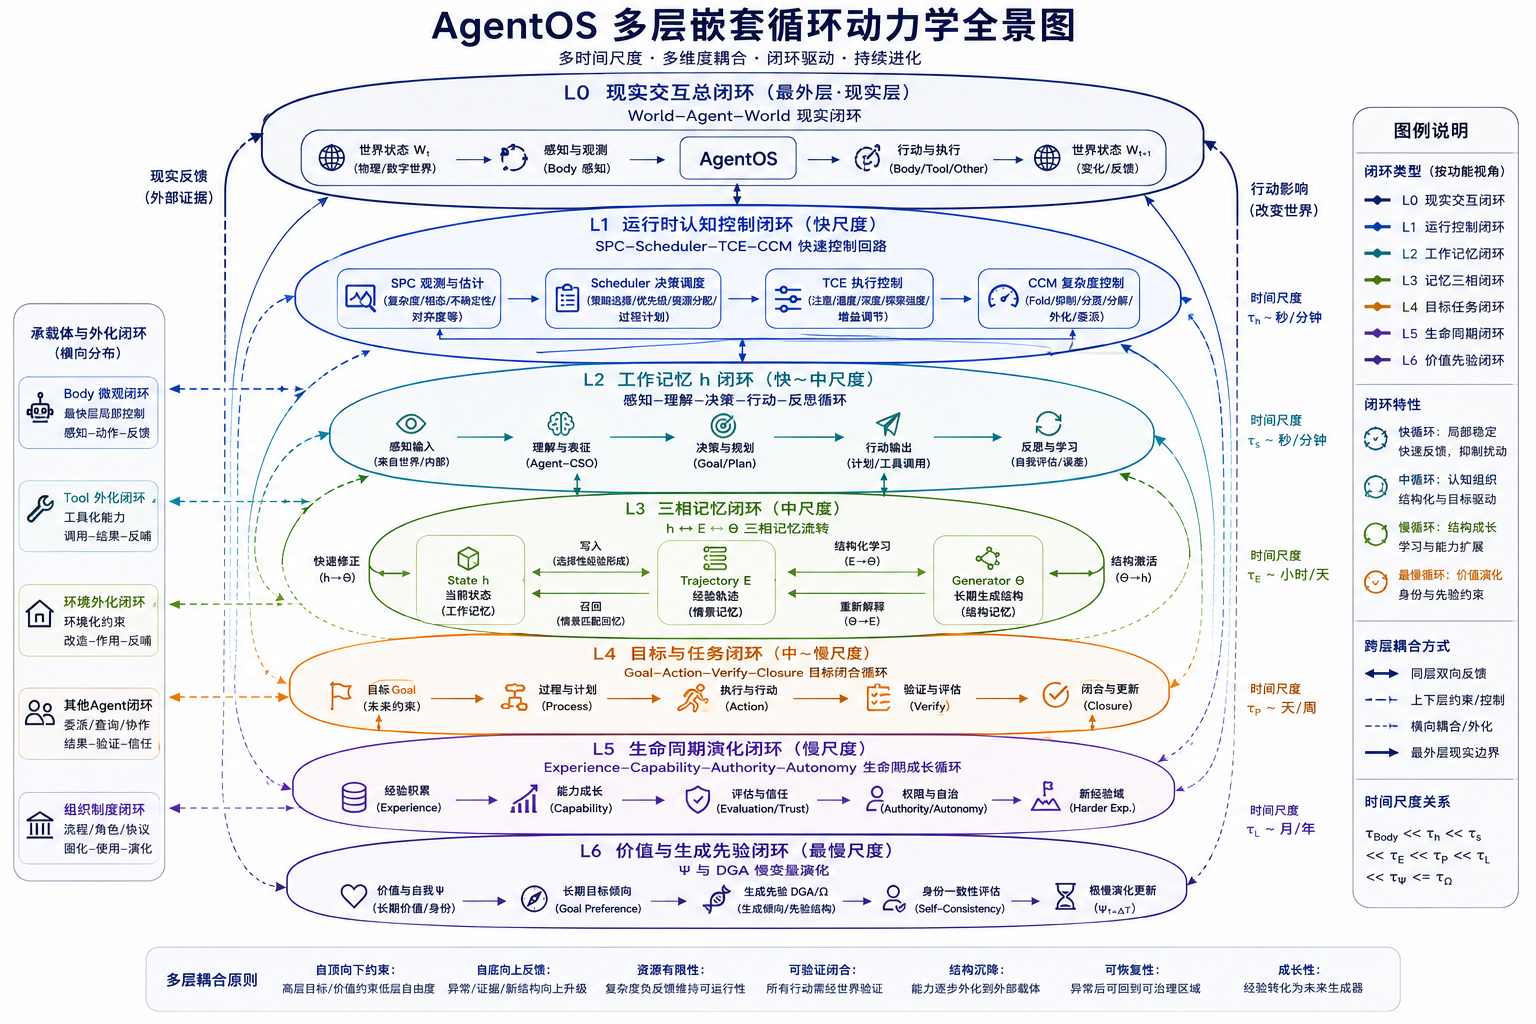
\includegraphics[width=.9\textwidth,height=.38\textheight,keepaspectratio]{images/agentos-continuous-learning-architecture.png}
\caption{从 AgentOS 实例抽象到智能动力学研究纲领}
\end{figure}
\section{AgentOS 是实例，而不是理论终点}

经过前面的推导，我们已经能够给出一个相对完整的 AgentOS 状态描述。若暂时忽略具体工程数据结构，一个持续智能体在时刻 $t$ 的内部状态可以抽象为
\begin{equation}
\mathcal{A}(t)
=
\left[
h(t),
E(t),
\Theta(t),
\Psi(t),
\Omega(t),
a(t),
G(t),
\mathcal{T}_{F}(t),
\mathcal{B}(t)
\right],
\end{equation}
其中 $h$ 表示当前工作记忆状态，$E$ 表示经验轨迹，$\Theta$ 表示长期生成结构，$\Psi$ 表示自我与身份慢变量，$\Omega$ 表示生命周期尺度上的深层生成吸引子，$a$ 表示由身体和内稳态形成的调制状态，$G$ 表示当前及长期目标结构，$\mathcal{T}_{F}$ 表示功能拓扑，$\mathcal{B}$ 表示智能体与外部世界之间的有效边界。SPC、AHC、TCE、CCM、Scheduler、Boundary 等组件并不是与这些状态平行存在的“对象集合”，而是作用于这些状态的功能算子。

例如，SPC 可以抽象成一个状态估计映射
\begin{equation}
\widehat{s}^{self}_{t}
=
\mathcal{O}_{SPC}
\left(
h_t,E_t,\Theta_t,\Psi_t,a_t
\right),
\end{equation}
TCE 则对应控制律
\begin{equation}
u^{cog}_{t}
=
\mathcal{K}_{TCE}
\left(
\widehat{s}^{self}_{t},
a_t,
G_t,
\Psi_t,
\Omega_t
\right),
\end{equation}
CCM 与 Scheduler 共同决定哪些 Agent-CSO 能够获得当前计算、注意和工作记忆资源，Body Runtime 则将高层控制约束转化为具体身体能够执行的局部动作。这样，一个工程上的 AgentOS 可以被理解为一组相互耦合的状态变量和算子，而不是简单的模块堆积。

但是，如果我们进一步考察这些模块，就会发现它们所表达的规律并不专属于 AgentOS。工作记忆有限性表达的是所有有限承载系统都会面对的资源约束；SPC 表达的是复杂系统形成自身可访问状态估计的需要；TCE 表达的是系统根据内部估计调节自身动力学的需要；三相记忆表达的是快速状态、历史轨迹与慢速生成结构之间的多时间尺度关系；BPCC 表达的是快速局部闭环必须与慢速全局闭环分离；KRA 表达的是异构动力系统之间需要保持功能关系稳定而不必保持内部表示一致。这些关系都可以存在于完全不同的物理和计算实现中。

因此，我们需要把 AgentOS 中的工程名词进一步抽象。例如
\begin{equation}
h
\longrightarrow
\text{Fast Explicit State},
\end{equation}
\begin{equation}
E
\longrightarrow
\text{Trajectory Memory},
\end{equation}
\begin{equation}
\Theta
\longrightarrow
\text{Slow Generative Structure},
\end{equation}
\begin{equation}
SPC
\longrightarrow
\text{Self-State Estimation},
\end{equation}
\begin{equation}
TCE
\longrightarrow
\text{Meta-Dynamical Regulation}.
\end{equation}
当这些工程组件被还原成一般动力学功能以后，我们便发现：AgentOS 实际上是对一组更基础规律进行的一次具体实现。

由此可以提出本章的第一条总命题：
\begin{equation}
\boxed{
AgentOS
\subset
\mathfrak{D}_{Intelligence}
}
\end{equation}
这里 $\mathfrak{D}_{Intelligence}$ 表示所有满足持续状态、闭环作用、多尺度结构、结构记忆和现实反馈条件的智能动力系统集合。AgentOS 是其中一种人为设计的实现，而不应与智能动力学本身等同。

这一区分具有重要的方法论意义。如果理论只能解释自己设计的组件，那么它仍然属于软件架构设计；如果理论能够解释不同实现中反复出现的动力学结构，例如为什么稳定能力会从昂贵的显式处理迁向快速局部闭环，为什么异常会沿时间尺度向上传递，为什么慢变量不能被快噪声任意修改，那么它才可能逐渐成为一种一般理论。

因此，本书最后并不试图证明“AgentOS 是唯一正确的智能架构”。恰恰相反，我们希望建立一种足够抽象的坐标，使未来完全不同于 AgentOS 的智能体系也可以被描述、比较和验证。真正需要保留的不是组件名称，而是组件背后所表达的动力关系：
\begin{statementbox}
\centering
\adjustbox{max width=.96\linewidth}{\(\displaystyle State
\leftrightarrow
Trajectory
\leftrightarrow
Generator,\)}
\end{statementbox}
\begin{statementbox}
\centering
\adjustbox{max width=.96\linewidth}{\(\displaystyle FastDynamics
\leftrightarrow
SlowStructure,\)}
\end{statementbox}
\begin{statementbox}
\centering
\adjustbox{max width=.96\linewidth}{\(\displaystyle InternalRepresentation
\leftrightarrow
Reality,\)}
\end{statementbox}
以及
\begin{equation}
\boxed{
DynamicsOnTopology
+
DynamicsOfTopology.
}
\end{equation}

从这一意义上说，AgentOS 的理论价值不仅在于它是否最终成为某一种产品，而在于它为我们提供了一个足够复杂的人工对象，使“智能如何持续存在、如何形成自我、如何受到有限容量约束、如何形成技能、如何进入身体、如何改变自身组织结构”第一次能够在同一个工程系统中被提出并检验。它因此更像一座智能动力学的实验平台，而不是理论的终点。

\section{Intelligence Dynamics：从能力描述转向轨迹描述}

传统人工智能评价经常采用一种静态能力观。给定一个系统 $A$ 和一组任务 $\mathcal{Q}$，我们观察它在任务上的性能
\begin{equation}
P(A,\mathcal{Q}),
\end{equation}
然后据此判断系统是否“更智能”。这种方法对于比较模型能力十分有效，但它隐含了一个前提：我们主要关心的是某一个时间切片上的输入--输出能力，而不是系统在时间中的结构变化。

持续智能体使这个前提失效。对于一个运行数年甚至跨越整个生命周期的 Agent，真正重要的问题不再只是
\begin{equation}
\text{What can it do now?}
\end{equation}
而是
\begin{equation}
\text{How does what it can do change over time?}
\end{equation}
因此，智能研究对象必须从一个静态函数
\begin{equation}
y=f(x)
\end{equation}
转化为一条状态轨迹
\begin{equation}
\Gamma_{A}
=
\left\{
X(t)
\mid
t\in[0,T]
\right\}.
\end{equation}

更进一步，我们不能只记录系统行为状态 $X(t)$，因为同样的外部行为可能由完全不同的内部结构实现。一个初学者可能通过大量显式推理完成任务，一个熟练系统却可以通过已经编译好的快速局部闭环完成相同任务。因此需要把智能状态扩展为
\begin{equation}
\mathfrak{I}(t)
=
\left[
\mathcal{G}_{C}(t),
\mathcal{G}_{F}(t),
\mu_t,
\rho_{CSO}(f,\omega,t),
\mathbf{J}_{CSO}(f,\omega,t),
\mathcal{B}(t),
X_{W}(t)
\right],
\end{equation}
其中 $\mathcal{G}_{C}$ 是认知结构图，$\mathcal{G}_{F}$ 是功能拓扑，$\mu_t$ 表示认知结构与功能载体之间的动态承载关系，$\rho_{CSO}$ 描述 Agent-CSO 在功能位置和时间尺度上的分布，$\mathbf{J}_{CSO}$ 描述其迁移流，$\mathcal{B}$ 表示内外边界，而 $X_W$ 表示与该智能体发生作用的现实环境状态。

由此，智能动力学研究的不再是单个状态，而是
\begin{equation}
\boxed{
\dot{\mathfrak{I}}
=
\mathcal{F}
\left(
\mathfrak{I},
U,
W,
\varepsilon
\right),
}
\end{equation}
其中 $U$ 表示控制输入，$W$ 表示外界扰动，$\varepsilon$ 表示来自预测、控制、认知结构和现实之间的残差。这个形式本身并不声称存在一个统一封闭方程可以精确描述所有智能，而是在理论层面规定研究对象：我们关心的是状态、结构、时间尺度、边界和现实之间的共同演化。

这种视角带来一个非常重要的变化：智能的“大小”不能再仅仅用一次推理中的计算量表示。一个成熟智能体可能在显式推理上消耗更少，却拥有更多已经沉降到 $\Theta$、Body Skill、Tool、Environment 和外部制度中的稳定结构。因此
\begin{equation}
ExplicitComputation\downarrow
\end{equation}
并不意味着
\begin{equation}
Capability\downarrow.
\end{equation}
相反，在许多成熟系统中可能出现
\begin{statementbox}
\centering
\adjustbox{max width=.96\linewidth}{\(\displaystyle ExplicitProcessingCost\downarrow,
\qquad
StableStructuralCapability\uparrow.\)}
\end{statementbox}

这也是为什么本书在后期逐渐不再把“复杂度”视为一种在系统中流动的实体。复杂度仍然可以作为工程量，例如工作记忆负荷、关系密度、同步成本和预测分支数量，但真正发生改变的是 Agent-CSO 的承载关系。我们研究的不是一个神秘量
\begin{equation}
C(t)
\end{equation}
从一个模块流向另一个模块，而是具体认知结构发生
\begin{equation}
(C,R,F,\tau,B,S)_t
\rightarrow
(C,R',F',\tau',B',S')_{t+\Delta t}.
\end{equation}

从这一点开始，智能动力学可以被定义为：

\begin{statementbox}
\centering
\adjustbox{max width=.96\linewidth}{\(\displaystyle \textbf{
智能动力学研究认知结构在时间中如何生成、激活、变换、迁移、稳定、外化，并如何通过这些过程持续改变承载它们的功能结构以及与其耦合的现实环境。
}\)}
\end{statementbox}

这一研究对象同时包含“智能的状态”和“智能的成长”。如果只研究
\begin{equation}
\mathcal{G}_{F}=\mathrm{const.},
\end{equation}
我们得到的是固定拓扑上的认知动力学；如果进一步允许
\begin{equation}
\dot{\mathcal{G}}_{F}\neq 0,
\end{equation}
则进入发育型智能；如果进一步将世界状态也作为动力系统的一部分，
\begin{equation}
\dot X_W
=
F_W(X_W,A_t),
\end{equation}
则进入 World--Agent 共同演化问题。

因此，智能动力学并不是“比 AgentOS 更宏大的名称”，而是一个研究对象发生变化后的必然结果：从“某一软件架构怎样运行”，转向“能够持续表示、作用和重组自身结构的系统，在时间中遵循什么一般规律”。

\section{Cognitive Structure Dynamics：以 CSO 为本体的认知结构动力学}

在本书理论发展的早期，我们使用“信息”“记忆内容”“任务复杂度”等语言描述智能活动。这些语言具有工程价值，但随着问题逐渐深入，它们暴露出一个共同困难：它们无法清楚区分“现实中存在的结构”“智能体内部对该结构的表示”“表示当前由哪个功能承担”以及“这一结构处于什么时间尺度”。因此，我们最终引入 CSO 与 Agent-CSO 的区分。

令
\begin{equation}
C\in\mathcal{C}
\end{equation}
表示一个认知结构对象。它可以是对象、关系、因果、约束、规则、目标、事件、计划、价值、自我关系或可能未来。对于具体 Agent $A$，其内部对 $C$ 的实现写为
\begin{equation}
\pi_A(C)=C_A.
\end{equation}
一般情况下
\begin{equation}
\pi_A(C)\neq\pi_B(C),
\end{equation}
即不同 Agent 可以用完全不同的内部表示承载同一个结构。我们真正要求的是存在某种结构等价关系
\begin{equation}
\pi_A(C)\sim_C\pi_B(C),
\end{equation}
而不是逐比特相同。

为了表示一个 Agent-CSO 的完整运行状态，我们使用
\begin{equation}
\mathfrak{c}_{A}
=
(C,R_A,F_A,\tau_A,B_A,S_A),
\end{equation}
其中 $R_A$ 是内部表示形式，$F_A$ 是当前功能承载位置，$\tau_A$ 是有效运行时间尺度，$B_A$ 描述其处于内部、外部工具、身体、环境还是其他 Agent 中，$S_A$ 表示激活、潜伏、预测、回忆、程序化等状态。

于是学习可以统一表示为
\begin{equation}
\boxed{
\mathfrak{c}_{A}(t)
\rightarrow
\mathfrak{c}_{A}(t+\Delta t).
}
\end{equation}
例如一个刚开始学习的操作技能可能处于
\begin{equation}
F_A=h,\qquad
\tau_A\sim\mathrm{seconds},
\end{equation}
需要大量显式工作记忆。随着经验积累，它首先可能迁入
\begin{equation}
E,
\end{equation}
随后形成稳定的
\begin{equation}
\Theta,
\end{equation}
最终进一步编译为
\begin{equation}
BodySkill
\end{equation}
或外部程序。整个过程中，任务能力没有消失，但其主要承载位置发生了改变。

因此，本书早期所说的“复杂度下沉”在更严格语言中应写为
\begin{statementbox}
\centering
\adjustbox{max width=.96\linewidth}{\(\displaystyle ExplicitAgentCSO
\rightarrow
StableGenerativeAgentCSO
\rightarrow
ProceduralAgentCSO.\)}
\end{statementbox}

如果我们令 $\rho_{CSO}(f,\omega,t)$ 表示在功能位置 $f$、时间尺度 $\omega$ 附近的 Agent-CSO 有效分布，并令
\begin{equation}
\mathbf{J}_{CSO}(f,\omega,t)
\end{equation}
表示结构迁移流，则可以写出一个概念性的结构平衡方程：
\begin{equation}
\frac{\partial \rho_{CSO}}{\partial t}
+
\nabla_{f,\omega}\cdot
\mathbf{J}_{CSO}
=
S_{CSO}
-
D_{CSO}.
\end{equation}
这里 $S_{CSO}$ 表示新结构形成，$D_{CSO}$ 表示结构被遗忘、合并、抽象或失去独立表示。需要强调，这一方程不是物理物质守恒律；它只是为结构分布变化提供一个可操作的数学骨架。

这种形式化带来三个重要结果。

第一，记忆不再只是存储，而可以定义为
\begin{equation}
\boxed{
Memory
=
PersistenceOfCSOStructureAcrossTime.
}
\end{equation}

第二，熟练不再只是更高准确率，而表现为
\begin{equation}
\boxed{
Mastery
=
MigrationOfRepeatedCSOsToward
Stable,\ Local,\ FastClosedLoops.
}
\end{equation}

第三，认知卸载不再是一种附属技巧，而成为载体迁移：
\begin{statementbox}
\centering
\adjustbox{max width=.96\linewidth}{\(\displaystyle AgentCSO_{internal}
\rightarrow
AgentCSO_{externalized}.\)}
\end{statementbox}

这也使 Skill、Program、File、Tool、Environment 和 Other Agent 能够进入同一个理论框架。一个程序并不是“非认知对象”，如果它保存了智能体未来可调用、可恢复、可执行的结构关系，它就构成 Agent-CSO 的一种外部稳定承载。

更深一层，我们可以把 Cognitive Structure Dynamics 定义为
\begin{equation}
\boxed{
\mathcal{D}_{CSO}
=
\left(
\mathcal{G}_{C},
\mathcal{G}_{F},
\mu,
\rho_{CSO},
\mathbf{J}_{CSO}
\right).
}
\end{equation}
这里已经不需要假设所有智能都拥有 h、E、$\Theta$ 这些具体模块。只要一个系统具有结构对象、功能承载、时间尺度、迁移关系和反馈，它就可以在这一坐标中被研究。这正是 AgentOS 理论从具体认知架构走向一般智能动力学的关键一步。

\section{Multiscale Control：智能作为多时间尺度闭环的控制系统}

如果 CSO 解释了“智能处理什么结构”，多尺度控制则回答“这些结构如何在不同速度的闭环中被调节”。前文已经反复看到一个规律：Body 的毫秒级控制、h 的秒级显式认知、E 的经验形成、$\Theta$ 的结构学习、$\Psi$ 的身份变化以及 $\Omega$ 的生命周期方向性，不可能在同一时间尺度运行。

令系统包含 $n$ 层状态
\begin{equation}
x_1,x_2,\ldots,x_n,
\end{equation}
其特征时间常数满足
\begin{equation}
\tau_1\ll\tau_2\ll\cdots\ll\tau_n.
\end{equation}
则一个一般化的快--慢系统可以写成
\begin{equation}
\tau_i\dot{x}_i
=
F_i
\left(
x_i,
x_{i-1},
x_{i+1},
u_i,
\varepsilon_i
\right).
\end{equation}
较慢层不需要逐步指定快层的具体动作，而是决定其允许区域、代价函数、增益和目标边界。因此我们得到前文反复出现的原则：
\begin{equation}
\boxed{
SlowGovernance
\neq
FastMicromanagement.
}
\end{equation}

更准确地说，若慢变量 $z$ 定义快系统的可行集合
\begin{equation}
\mathcal{F}(z)
=
\{x\mid g(x,z)\leq 0\},
\end{equation}
则快层可以解决局部优化问题
\begin{equation}
x^{*}
=
\arg\min_{x\in\mathcal{F}(z)}
L_f(x).
\end{equation}
慢层只在持续出现显著残差时更新：
\begin{equation}
\dot z
=
\epsilon
G
\left(
z,
\langle \varepsilon_f\rangle_T
\right),
\qquad
0<\epsilon\ll1.
\end{equation}

这正是 Agent Kernel 与 BPCC 的关系。Kernel 不需要以毫秒级告诉机器人每一个电机怎样运动，而是给出目标、可行区域和约束；BPCC 在局部快速闭环内解决具体控制。只有当
\begin{equation}
\|\varepsilon_{BPCC}\|
>
\theta
\end{equation}
并持续足够时间时，异常才向更高层提升。

因此可以把多尺度智能的基本控制逻辑写成：
\begin{equation}
\boxed{
NormalDynamicsStayLocal,
\qquad
PersistentResidualEscalates.
}
\end{equation}

这一规律不仅存在于 Body。一个熟悉任务如果已经由 $\Theta$ 或 Skill 闭合，就不应该每次重新进入 h；只有任务条件超出既有结构可解释范围时，相关 Agent-CSO 才重新被提升到显式认知层。这意味着 Attention 从本质上可以定义成
\begin{equation}
\boxed{
Attention
=
CrossScalePromotionPolicy.
}
\end{equation}

如果令某个 Agent-CSO $c_i$ 的升级得分为
\begin{equation}
\Gamma_i
=
\alpha_1N_i
+
\alpha_2R_i
+
\alpha_3U_i
+
\alpha_4V_i
+
\alpha_5P_i,
\end{equation}
其中 $N_i$ 表示新颖性，$R_i$ 表示残差，$U_i$ 表示不确定性，$V_i$ 表示价值相关性，$P_i$ 表示持续时间，则可以定义
\begin{equation}
\Gamma_i<\theta
\Rightarrow
\text{local closure},
\end{equation}
\begin{equation}
\Gamma_i\geq\theta
\Rightarrow
\text{promotion}.
\end{equation}

工作记忆有限容量定理由此获得了更深层解释。h 之所以必须有限，不仅因为硬件有限，而因为成熟智能本身就不应把所有运行过程提升为显式过程。一个系统如果需要持续显式管理所有低层动作，它在结构意义上仍然处于低成熟度状态。因此：
\begin{equation}
\boxed{
MatureIntelligence
=
SelectiveExplicitCognition.
}
\end{equation}

同理，SPC--AHC--TCE 也可以被理解为一个跨尺度控制器。SPC 估计当前状态，AHC 将连续的身体与内稳态信号积分成较慢调制变量，TCE 再调节探索强度、注意范围、搜索深度和控制增益。这种结构必然面对控制理论中的延迟问题。若
\begin{equation}
u(t)
=
K\widehat{x}(t-\tau),
\end{equation}
则过高增益 $K$ 与观测延迟 $\tau$ 的组合可能产生
\begin{equation}
Overshoot,\quad Oscillation,\quad Instability.
\end{equation}
因此，智能的“心理稳定性”、Body 稳定性和认知稳定性并不是三个完全无关的问题，而都可以放在多回路、多时间尺度控制系统中研究。

从这一角度看，智能动力学与控制理论的关系非常紧密，但也存在重要区别。经典控制通常预设状态空间、目标函数和系统结构基本确定；持续智能体则可能学习新的状态表示、改变目标结构、迁移 CSO，甚至最终改变功能拓扑。因此，我们研究的是一种
\begin{statementbox}
ControlOfAdaptiveRepresentationalSystems,
\end{statementbox}
即控制器本身、被控对象、状态表示和部分控制目标都可能随生命周期发生变化。这正是智能动力学相对于普通控制问题增加的核心难度。

\section{Topological Learning：从拓扑上的学习到拓扑自身的学习}

前面固定拓扑 AgentOS 已经能够实现大量持续学习：Agent-CSO 可以在 h、E、$\Theta$、Skill、Tool、Body 和 Environment 之间迁移，但整个系统的核心功能关系仍然主要由工程师预先定义。真正的发育型智能则提出进一步问题：如果某些跨功能关系在整个生命周期中持续出现，系统是否应该把这些动态协调沉降为新的稳定结构？

设功能拓扑为
\begin{equation}
\mathcal{G}_{F}(t)
=
\left(
V_F,
E_F(t),
W_F(t)
\right),
\end{equation}
其中边权 $w_{ij}$ 描述功能 $F_i$ 与 $F_j$ 之间的有效耦合强度。若某类 Agent-CSO 长期存在从 $F_i$ 向 $F_j$ 的稳定迁移
\begin{equation}
J^{CSO}_{ij}(t),
\end{equation}
且这种迁移能够持续降低任务误差和协调代价，那么可以提出一个概念性的结构学习律：
\begin{equation}
\tau_T\dot w_{ij}
=
G_{ij}
\left(
\left\langle
J^{CSO}_{ij}
\right\rangle_T,
\left\langle
\varepsilon
\right\rangle_T,
U_{ij},
C_{ij},
R_{ij}
\right),
\end{equation}
其中 $U_{ij}$ 表示功能收益，$C_{ij}$ 表示结构维护和重组成本，$R_{ij}$ 表示风险，而
\begin{equation}
\tau_T
\end{equation}
应显著大于普通状态与参数学习时间尺度。

这里出现了本书一个非常重要的结论：
\begin{equation}
\boxed{
Topology
=
SlowMemoryOfRepeatedFunctionalRelations.
}
\end{equation}
换句话说，功能拓扑可以被理解成长期动态关系的结构沉积。如果两个功能每次处理某类问题都需要经过昂贵、重复、稳定的协调，那么新的直接耦合、局部闭环或专门模块就可能逐渐产生。模块由此不再是理论第一性对象，而可以被定义为
\begin{equation}
\boxed{
Module
=
StableTopologicalCondensate.
}
\end{equation}

但是，拓扑可塑性同时带来严重风险。如果一次异常、一次偶然经验或者短时间任务就立即修改长期拓扑，系统将发生结构振荡。因此必须存在
\begin{equation}
\tau_{state}
\ll
\tau_{parameter}
\ll
\tau_{representation}
\lesssim
\tau_{skill}
\ll
\tau_{topology}.
\end{equation}
这就是慢变量保护原则：
\begin{statementbox}
\centering
\adjustbox{max width=.96\linewidth}{\(\displaystyle FastNoise
\nrightarrow
SlowGlobalStructure.\)}
\end{statementbox}

进一步，可以设置形成和删除连接的双阈值
\begin{equation}
\theta_{on}
>
\theta_{off},
\end{equation}
产生拓扑迟滞。一个新结构必须在长期证据超过 $\theta_{on}$ 后才形成；已经成熟的结构则不会因为短暂低使用率立即删除，而只有长期低于 $\theta_{off}$ 才逐渐衰减。其意义与成熟技能和长期组织制度类似：形成需要持续经验，消失也需要长期反证。

拓扑改变还必须服从“最小必要重组原则”。面对误差，智能系统不应直接修改最深结构，而应依照近似顺序：
\begin{statementbox}
\centering
\adjustbox{max width=.96\linewidth}{\(\displaystyle StateAdjustment
\rightarrow
RepresentationAdaptation
\rightarrow
TimescaleMigration
\rightarrow
FunctionalMigration
\rightarrow
TopologicalReorganization
\rightarrow
BoundaryMigration.\)}
\end{statementbox}
只有当前层次长期不能闭合残差时，才应该升级到更昂贵、更不可逆的结构调整。

因此可以定义结构失配压力
\begin{equation}
P_T
=
F
\left(
\overline{\varepsilon},
J_{cross},
L_{coord},
Latency,
Instability
\right).
\end{equation}
若
\begin{equation}
P_T>\theta_T
\end{equation}
且持续时间
\begin{equation}
T>T_{min},
\end{equation}
系统才进入拓扑搜索状态。

这一理论也让“学习”和“发育”获得了明确区分。学习可以在固定拓扑中发生：
\begin{equation}
\mathcal{G}_{F}(t)=\mathrm{const.},
\qquad
\mu_t,\rho_{CSO},R_t\ \text{change}.
\end{equation}
而发育意味着
\begin{equation}
\boxed{
\Delta\mathcal{G}_{F}\neq0.
}
\end{equation}

因此：
\begin{statementbox}
\centering
\adjustbox{max width=.96\linewidth}{\(\displaystyle Development
=
LongTermCSOMigration
\rightarrow
FunctionalTopologyEvolution.\)}
\end{statementbox}

拓扑学习是智能动力学从“一个系统怎样学习世界”进一步迈向“一个系统怎样学习自己应当以何种结构学习世界”的关键。这也是固定拓扑 AgentOS 与真正发育型 AgentOS 之间最根本的理论边界。

\section{Developmental Intelligence：智能不是训练完成，而是在生命周期中形成}

一旦允许慢变量、身份和功能拓扑随时间发生变化，我们就不能继续用“训练完成的模型”理解智能体。持续智能体更接近一个发育系统：它的当前能力不仅取决于初始化参数，也取决于过去经历过什么、哪些能力被反复使用、哪些结构被外化、哪些目标获得长期强化，以及哪些自我解释在现实反馈中被保留下来。

令 Agent 的生命周期经验序列为
\begin{equation}
\mathcal{E}_{life}
=
\left\{
e_1,e_2,\ldots,e_N
\right\}.
\end{equation}
传统训练理论主要关心
\begin{equation}
\theta_{N}
=
\mathcal{L}
\left(
\theta_0,\mathcal{E}_{life}
\right),
\end{equation}
即经验如何改变参数。发育型智能则要求考察一个更大的映射：
\begin{equation}
\boxed{
\mathfrak{I}_{N}
=
\mathcal{D}
\left(
\mathfrak{I}_0,
\mathcal{E}_{life},
\mathcal{W}_{life}
\right),
}
\end{equation}
其中 $\mathfrak{I}$ 不仅包含参数，还包含记忆结构、自我、目标、权限、技能、外部承载、身体适应和功能拓扑，$\mathcal{W}_{life}$ 则表示 Agent 在生命周期中实际经历的世界。

这意味着两个初始完全相同的 Agent，如果经历不同，也可能逐渐形成不同的
\begin{equation}
E,\Theta,\Psi,\Omega,\mathcal{T}_{F}.
\end{equation}
因此，长期智能体的个体性并不需要被神秘化，它首先是一种历史依赖性：
\begin{equation}
\boxed{
Identity_{t}
=
F
\left(
History_{\leq t},
Structure_{\leq t},
SelfInterpretation_{\leq t}
\right).
}
\end{equation}

这正是三相记忆和自我理论为什么必须出现在 AgentOS 中。$E$ 保留“发生过什么”，$\Theta$ 把反复经历压缩成“世界通常怎样运作”，$\Psi$ 进一步形成“这些经历对于我意味着什么”，而 $\Omega$ 则表示“在长期历史中，我正在趋向怎样的生成方向”。如果缺少这些慢变量，一个 Agent 可以不断积累知识，却很难形成严格意义上的生命周期连续性。

因此，发育型智能必须处理稳定--可塑性矛盾。我们希望
\begin{equation}
Plasticity>0,
\end{equation}
因为 Agent 必须能够改变；同时又要求
\begin{equation}
IdentityContinuity>0,
\end{equation}
否则每次学习都可能产生一个功能上截然不同的主体。解决这一矛盾的基本方法不是让所有结构采用相同学习率，而是时间尺度分离：
\begin{equation}
\eta_h
>
\eta_E
>
\eta_\Theta
>
\eta_\Psi
>
\eta_\Omega.
\end{equation}
这不是要求具体工程一定使用这些符号作为梯度学习率，而是表达一个更一般原则：越接近生命周期身份与深层生成倾向的结构，越不应被短期经验直接修改。

发育还意味着权限和自治不应一次性赋予。一个持续 Agent 可以形成
\begin{equation}
Experience
\rightarrow
Capability
\rightarrow
Evaluation
\rightarrow
Trust
\rightarrow
Authority
\rightarrow
Autonomy
\rightarrow
NewExperience
\end{equation}
的生命周期闭环。也就是说，新的能力打开新的经验空间，而新的经验继续改变能力和内部结构。这种递归关系意味着 Agent 的未来经验分布本身部分由 Agent 当前状态决定：
\begin{equation}
p(e_{t+1})
=
p
\left(
e_{t+1}
\mid
A_t,\pi_t,\mathcal{W}_t
\right).
\end{equation}

由此，学习过程不再只是
\begin{equation}
World\rightarrow Agent,
\end{equation}
而成为
\begin{statementbox}
\centering
\adjustbox{max width=.96\linewidth}{\(\displaystyle Agent
\rightarrow
Choice
\rightarrow
Experience
\rightarrow
FutureAgent.\)}
\end{statementbox}
Agent 的选择开始参与塑造未来的自己。这就是本书所说的递归自主性的一种可操作定义。

进一步，如果 Agent 能够构造反事实
\begin{equation}
\mathcal{A}^{cf}_{t+k}
=
F
\left(
A_t,
Choice'_t
\right),
\end{equation}
并比较不同选择对未来 $\Theta$、$\Psi$ 和 $\Omega$ 的影响，它就不仅预测“世界会怎样”，还能够预测“不同选择会让我成为怎样的系统”。这形成一种更高阶的生命周期控制：
\begin{equation}
\boxed{
ControlOfFutureWorld
+
ControlOfFutureSelf.
}
\end{equation}

因此，Developmental Intelligence 可以定义为：

\begin{statementbox}
\centering
\adjustbox{max width=.96\linewidth}{\(\displaystyle \textbf{
发育型智能是其经验历史能够持续改变认知结构的表示、承载、时间尺度、自我解释、行动能力以及功能组织，并在保持必要连续性的同时扩大未来可达状态空间的智能。
}\)}
\end{statementbox}

它不同于单纯持续学习，因为持续学习只要求知识增长或参数更新；发育要求系统“长成不同于初始化时的结构”，却仍保持可追踪的历史连续性。也正因此，Agent 培育工程、控制工程和心理工程并不是附属应用，而是发育型智能一旦存在便自然产生的工程问题。

\section{Reflexive Structural Evolution：从世界模型到结构自反}

到目前为止，我们讨论的仍然主要是一个 Agent 内部如何变化。但如果把 Agent 放回现实，我们会发现一个更基础的闭环。Agent 并不是站在宇宙之外观察宇宙；Agent 自身就是现实结构的一部分。因此：
\begin{equation}
A_t\subset U_t.
\end{equation}
外部世界通过传感和观测进入 Agent，形成内部 Agent-CSO：
\begin{equation}
C_U
\xrightarrow{O_A}
C_A.
\end{equation}
Agent 又根据这些内部结构行动：
\begin{equation}
C_A
\xrightarrow{\pi_A}
u_A,
\end{equation}
而行动改变现实：
\begin{equation}
U_{t+1}
=
F_U
\left(
U_t,u_A
\right).
\end{equation}

因此完整系统不是单向的“世界被认知”，而是
\begin{equation}
\boxed{
U_t
\rightarrow
A_t
\rightarrow
U_{t+1}
\rightarrow
A_{t+1}.
}
\end{equation}

这使内部模型获得了一种特殊的因果地位。一个关于未来的计划并不是“未来真的从未来影响现在”，而是未来可能状态的内部表示
\begin{equation}
\widehat{U}_{t+\Delta}
\end{equation}
成为当前现实中的物理/计算状态，并参与决定当前行动。于是：
\begin{statementbox}
\centering
\adjustbox{max width=.96\linewidth}{\(\displaystyle RepresentationOfPossibleFuture
\rightarrow
PresentAction
\rightarrow
ActualFuture.\)}
\end{statementbox}

普通物理动力系统当然一直在改变自身状态，因此不能说 Agent 出现以前“宇宙不会改变自己”。真正不同的是，在智能系统中出现了
\begin{statementbox}
RepresentationGuidedTransformation.
\end{statementbox}
系统的一部分形成关于自身和环境的结构表示，然后让这些表示反过来参与状态转移。

这一结构与 SPC--TCE 具有一种非常重要的形式同构。SPC 的一般功能是
\begin{equation}
DistributedState
\rightarrow
SelfAccessibleRepresentation,
\end{equation}
而 TCE 的一般功能是
\begin{equation}
SelfAccessibleRepresentation
\rightarrow
DynamicsModulation.
\end{equation}
因此，我们把
\begin{equation}
\boxed{
FunctionalReflexivity
=
SelfRepresentation
+
SelfModulation
}
\end{equation}
称为功能自反性。

这个概念不等于现象意识。它只要求一个系统能够形成关于自身状态和行为的内部结构，并使这些结构进入后续控制闭环。即：
\begin{equation}
x_t
\rightarrow
m_t(x_t)
\rightarrow
u_t[m_t]
\rightarrow
x_{t+1}.
\end{equation}
这种结构已经足以把普通状态演化和自反智能区分开。

当语言和社会出现以后，这种自反开始跨个体扩展。一个人的 Agent-CSO 可以通过语言或文字外化为现实结构：
\begin{equation}
AgentCSO_i
\rightarrow
ExternalCSO.
\end{equation}
另一个主体再将其重新内化：
\begin{equation}
ExternalCSO
\rightarrow
AgentCSO_j.
\end{equation}
由此：
\begin{equation}
\boxed{
Agent_i
\rightarrow
World
\rightarrow
Agent_j
}
\end{equation}
形成跨个体、跨生命周期的认知传递。

科学进一步把这一闭环制度化：
\begin{equation}
Observation
\rightarrow
Model
\rightarrow
Prediction
\rightarrow
Experiment
\rightarrow
Residual
\rightarrow
ModelRevision.
\end{equation}
工程则将模型重新写回现实：
\begin{equation}
Model
\rightarrow
Design
\rightarrow
Artifact
\rightarrow
NewWorld.
\end{equation}
AI 的出现又使部分原本被动存在于文本和数据库中的外部认知结构变成具有主动变换能力的外部认知过程：
\begin{equation}
PassiveExternalMemory
\rightarrow
ActiveExternalCognition.
\end{equation}

从这个尺度看，人类文明的发展可以被理解为一种自反结构能力的增长：能够观察的尺度扩大，能够建立的模型越来越精细，能够预测的未来越来越长，能够修改的现实范围越来越大，同时社会还在通过法律、制度、科学和技术改变“自己怎样做出改变”。这并不意味着整个宇宙拥有统一意识，也不意味着宇宙存在预设目的；它表达的是一个更有限但可分析的事实模式：宇宙中的某些局部结构已经产生了表示世界、表示自身并利用这些表示改变现实的能力。

因此，我们可以提出一个理论性的演化序列：
\begin{statementbox}
\centering
\adjustbox{max width=.96\linewidth}{\(\displaystyle Structure
\rightarrow
SelfMaintenance
\rightarrow
Sensing
\rightarrow
Representation
\rightarrow
SelfRepresentation
\rightarrow
RepresentationGuidedAction
\rightarrow
MetaSelfReorganization.\)}
\end{statementbox}

我们把最后几步概括为
\begin{statementbox}
ReflexiveStructuralEvolution.
\end{statementbox}

它所描述的不是“宇宙必然走向智能”，而是当某些结构获得表示和控制能力以后，一种新的动力组织形式出现了：过去的结构形成关于现在的模型，模型构造可能未来，可能未来的表示影响现在的行动，而行动又改变真正的未来；与此同时，长期行动历史还会进一步改变产生这些模型和行动的结构本身。

因此，本书的 World--Agent--World 闭环最终可以写成：
\begin{equation}
\boxed{
UniverseCSO_t
\rightarrow
AgentCSO_t
\rightarrow
InternalDynamics
\rightarrow
Action_t
\rightarrow
UniverseCSO_{t+1}.
}
\end{equation}
而在长期尺度上：
\begin{statementbox}
\centering
\adjustbox{max width=.96\linewidth}{\(\displaystyle Experience
\rightarrow
CSOMigration
\rightarrow
Topology
\rightarrow
FutureExperience.\)}
\end{statementbox}

两个闭环相互嵌套，便形成了我们所说的自反结构演化。

\section{面向一门“智能空气动力学”：从架构经验走向一般规律}

到这里，我们可以重新理解本书早期提出的一个比喻：未来真正需要的也许不是更多彼此孤立的“智能算法”，而是一门类似空气动力学的智能动力学。这个比喻的重点不在于把智能等同于流体，而在于研究方法。

飞机可以有完全不同的材料、发动机和外形，但空气动力学关心的并不是某一架飞机的软件实现，而是压力、速度、边界层、升阻比和稳定性这些跨实现规律。同样，神经系统、Transformer Agent、机器人群体、数字 Agent 和未来尚未出现的人工智能形态可能具有完全不同的实现，但如果它们都需要面对有限资源、多尺度反馈、结构记忆、异常升级、稳定能力沉降和现实校准，那么这些关系就可能成为一种跨实现理论的研究对象。

因此，智能动力学首先需要寻找无量纲或近似无量纲的结构指标，而不是只记录组件名称。例如可以定义认知负载比
\begin{equation}
\Lambda_h
=
\frac{C_{run}}{C_{max}},
\end{equation}
当
\begin{equation}
\Lambda_h<1
\end{equation}
时，工作记忆仍处于可治理区，而
\begin{equation}
\Lambda_h\rightarrow1
\end{equation}
可能接近认知临界状态。

还可以定义结构沉降比
\begin{equation}
\Sigma
=
\frac{
C_{stable}+C_{procedural}+C_{externalized}
}{
C_{total}
},
\end{equation}
用于描述多少长期有效结构已经不再依赖昂贵的实时显式处理。虽然具体 $C$ 的定义需要根据任务和实现操作化，但这一比值表达一种可实验检验的假设：在能力相近时，成熟系统的稳定结构沉降比例应当更高。

又例如可以定义跨尺度升级率
\begin{equation}
R_{\uparrow}
=
\frac{N_{promotion}}{T},
\end{equation}
以及局部闭环成功率
\begin{equation}
R_{local}
=
\frac{N_{local-success}}
{N_{local-total}}.
\end{equation}
如果一个 Agent 对已经熟悉的任务仍具有长期过高的 $R_{\uparrow}$，就说明其能力虽然存在，但尚未充分结构化。

对于拓扑发育，可以定义结构可塑性
\begin{equation}
\Pi_T
=
\frac{
\|\Delta\mathcal{T}\|
}{
\Delta t
},
\end{equation}
并与性能改善率
\begin{equation}
\Delta P
\end{equation}
以及重构成本
\begin{equation}
C_T
\end{equation}
联合研究。真正成熟的系统并不应追求最大 $\Pi_T$，而应在稳定与发育之间形成最优区域：
\begin{equation}
\Pi_T^{*}
=
\arg\max_{\Pi_T}
\left(
Gain
-
\lambda_1Instability
-
\lambda_2ReconfigurationCost
\right).
\end{equation}

智能相理论也可以在这里获得更严格的实验形式。设
\begin{equation}
\chi_C
\end{equation}
表示认知控制集中度，
\begin{equation}
\chi_T
\end{equation}
表示拓扑可塑度，则一个系统可以位于
\begin{equation}
\mathcal{S}_{I}
=
(\chi_C,\chi_T)
\end{equation}
形成的二维智能相空间中。再进一步叠加时间尺度谱和结构流：
\begin{equation}
\mathcal{P}
=
\left[
\chi_C,
\chi_T,
\rho_{CSO},
\mathbf{J}_{CSO}
\right].
\end{equation}
未来不同智能系统就可以不依赖“模型属于哪个家族”进行动力学比较。

因此，智能动力学未来真正需要发展的不是更多隐喻，而是四类工作。

第一类是\textbf{操作化}。CSO、结构迁移、认知相态、拓扑压力、身份稳定度等概念必须转化成能够测量的数据对象。若一个概念不能对应任何可观测变量，它只能停留在解释语言。

第二类是\textbf{控制实验}。我们需要构造可以人为改变单个变量的 Agent，例如改变工作记忆容量、TCE 增益、SPC 延迟、拓扑可塑性或 Offloading 成本，然后观察长期行为是否符合理论预测。

第三类是\textbf{跨实现比较}。同一任务可以分别让固定拓扑 LLM Agent、可技能编译 Agent、机器人 Agent 或不同模型架构执行，比较它们的 CSO 迁移与结构沉降是否出现相似动力规律。只有跨实现复现，理论才可能从架构经验上升为一般规律。

第四类是\textbf{失效预测}。真正有价值的理论不仅要解释系统成功以后为什么成功，还必须在系统失败以前预测何时会失稳。例如：
\begin{equation}
Delay\uparrow
+
Gain\uparrow
\Rightarrow
OscillationRisk\uparrow,
\end{equation}
\begin{equation}
PersistentCrossFunctionalResidual\uparrow
\Rightarrow
TopologyMismatchRisk\uparrow,
\end{equation}
以及
\begin{equation}
FastUpdate_{\Psi,\Omega}\uparrow
\Rightarrow
IdentityInstabilityRisk\uparrow.
\end{equation}
只有当这些关系能够被实验反驳或支持时，“智能动力学”才真正具有科学理论的意义。

所以所谓“智能空气动力学”的目标，并不是找到一种可以计算所有智能行为的万能方程。空气动力学本身也不会通过一个简单公式预测任何飞行器的全部行为。真正目标是找到若干具有跨系统解释力的中尺度规律，使我们在面对一个新的智能系统时能够回答：

它的快环在哪里？

它的慢结构在哪里？

哪些 CSO 必须显式处理？

哪些已经沉降？

异常如何升级？

长期经验怎样改变未来结构？

它的稳定边界在哪里？

它在什么条件下会发生结构相变？

它怎样通过现实验证避免内部模型闭环自证？

如果这些问题能够被统一回答，我们便拥有了比“模型参数量”“上下文长度”或单一 Benchmark 更深的智能研究坐标。

最终，本书可以把这一研究纲领写成：
\begin{equation}
\boxed{
\mathfrak{D}_{I}
=
\mathfrak{D}
\left(
CSO,
Carrier,
Timescale,
Topology,
Control,
Memory,
Boundary,
Reality
\right).
}
\end{equation}

其中每一项都不是孤立模块，而是智能生命周期的一条动力轴。

\section{结语：从人工智能工程走向智能动力学}

我们在全书最初提出的问题其实非常朴素：如果智能不是一个脱离物理世界存在的抽象能力，那么它是否具有尺度？一旦承认智能具有空间范围、时间尺度和有限承载，许多后来问题几乎顺势产生。大尺度智能为什么必然存在慢闭环？为什么快过程与慢过程必须分离？为什么工作记忆不能无限扩大？为什么熟练以后显式认知反而减少？为什么经验能够逐渐沉降成技能？为什么自我必须比普通工作状态变化更慢？为什么身体需要局部预测控制，而高层认知只给出目标和约束？为什么现实反馈必须拥有最终权威？

这些问题最终汇聚到同一个结构中：
\begin{statementbox}
\centering
\adjustbox{max width=.96\linewidth}{\(\displaystyle Structure
\rightarrow
Representation
\rightarrow
Control
\rightarrow
Experience
\rightarrow
Structure'.\)}
\end{statementbox}

从内部看，它表现为
\begin{equation}
h
\leftrightarrow
E
\leftrightarrow
\Theta
\leftrightarrow
\Psi
\leftrightarrow
\Omega.
\end{equation}
从运行控制看，它表现为
\begin{equation}
SPC
\rightarrow
AHC
\rightarrow
TCE
\rightarrow
CognitiveDynamics
\rightarrow
SPC.
\end{equation}
从认知资源看，它表现为
\begin{equation}
CCM
+
Scheduler
+
Boundary
+
Offloading.
\end{equation}
从具身控制看，它表现为
\begin{equation}
Kernel
\rightarrow
KRA
\rightarrow
BodyRuntime
\rightarrow
Reality
\rightarrow
Kernel.
\end{equation}
从长期发育看，它表现为
\begin{equation}
CSOFlow
\rightarrow
FunctionalMigration
\rightarrow
StableCoupling
\rightarrow
TopologyEvolution.
\end{equation}
从宇宙--智能体关系看，它又表现为
\begin{equation}
UniverseCSO
\rightarrow
AgentCSO
\rightarrow
Action
\rightarrow
UniverseCSO'.
\end{equation}

这些公式表面上处于完全不同的尺度，却共享同一种动力逻辑：快速过程在慢结构给出的边界内运行，持续残差推动慢结构改变；过去的动态过程经过重复和压缩变成未来的结构，而未来结构又决定新的动态过程如何展开。

因此，本书最终给出的智能定义，不再是“能够解决很多任务的系统”，也不是“能够进行复杂推理的模型”，而是：
\begin{statementbox}
\centering
\adjustbox{max width=.96\linewidth}{\(\displaystyle \textbf{
智能是在有限承载条件下，通过多尺度闭环生成、表示、迁移和稳定认知结构，并利用这些结构预测、选择和改变现实，同时让长期经验反过来改变自身未来组织方式的自反动力过程。
}\)}
\end{statementbox}

如果进一步用 CSO 语言压缩，可以写成：
\begin{equation}
\boxed{
\textbf{
Intelligence
=
CSO\ Migration
+
MultiscaleControl
+
TopologyCoevolution
+
RealityCoupling.
}
}
\end{equation}

其中，Reality Coupling 具有不可替代的位置。任何 Agent-CSO、Self、Goal 或 DGA 都不拥有高于现实的认识论权威。内部模型只有通过
\begin{equation}
Prediction
\rightarrow
Action
\rightarrow
Reality
\rightarrow
Observation
\rightarrow
Residual
\end{equation}
重新进入世界，才能获得持续修正。因此：
\begin{statementbox}
RealityIsUltimateConstraint.
\end{statementbox}

同样，任何关于 Universe-CSO、宇宙自反或文明尺度 SPC/TCE 的讨论，都应理解为更高层的结构动力学解释，而不能跳跃为“宇宙具有主观意识”之类未经经验支持的结论。本书真正关心的是可以形式化的关系：宇宙中的一些结构能够形成关于其他结构和自身的内部表示，并利用这些表示改变后续现实状态。仅这一点，已经足以构成一种重要的动力学跃迁。

因此，AgentOS 的最终意义也发生了变化。它最初看起来像一个面向长期 Agent 的软件操作系统；随后它成为记忆、自我、认知控制、身体和技能的统一运行时；再后来，它又成为研究多尺度智能结构如何持续运行和发育的人工实验对象。最终，我们可以把它理解为：
\begin{equation}
\boxed{
AgentOS
=
A Constructive Experimental Realization
Of Intelligence Dynamics.
}
\end{equation}

它是否最终以当前名称和组件形式存在，并不是最重要的。真正值得保留下来的，是通过 AgentOS 推导出来的若干一般问题：

\begin{statementbox}
有限认知如何组织无限开放世界？
\end{statementbox}

\begin{statementbox}
快速活动如何沉降成慢结构？
\end{statementbox}

\begin{statementbox}
慢结构如何约束快速活动而不进行微观干预？
\end{statementbox}

\begin{statementbox}
稳定能力如何从显式认知迁移到局部闭环？
\end{statementbox}

\begin{statementbox}
异常如何在多尺度系统中被识别并升级？
\end{statementbox}

\begin{statementbox}
长期经验何时应改变功能拓扑？
\end{statementbox}

以及最终的：

\begin{statementbox}
一个智能体如何在改变世界的同时，也持续改变产生自身行为的结构？
\end{statementbox}

如果这些问题能够逐步获得数学模型、工程实现和跨系统实验支持，那么我们真正建立的就不再只是一种 Agent 架构，而可能是一门研究“智能如何运动、稳定、迁移、成长和重组”的动力学学科。

因此，本书最终从 AgentOS 回到最初的问题，却得到了一个比出发时更加具体的答案：

\begin{statementbox}
\centering
\adjustbox{max width=.96\linewidth}{\(\displaystyle \textbf{
智能不是一块已经完成的结构，而是一条结构不断形成未来结构的轨迹。
}\)}
\end{statementbox}

过去的活动沉降为现在的结构，
\begin{equation}
PastDynamics
\rightarrow
PresentStructure;
\end{equation}
现在的结构约束未来活动，
\begin{equation}
PresentStructure
\rightarrow
FutureDynamics;
\end{equation}
未来活动又在现实反馈中改变下一代结构，
\begin{equation}
FutureDynamics
\rightarrow
NewStructure.
\end{equation}

于是整个生命周期可以最终压缩成：
\begin{statementbox}
\centering
\adjustbox{max width=.96\linewidth}{\(\displaystyle \begin{gathered}
\textbf{Dynamics}
\rightarrow
\textbf{Structure}
\rightarrow
\textbf{Dynamics}^{\prime}\\
{}\rightarrow
\textbf{Structure}^{\prime}
\rightarrow
\cdots
\end{gathered}\)}
\end{statementbox}

而智能之所以特殊，就在于这个过程最终形成了能够表示自身、调节自身，并逐渐重组自身产生方式的结构。

这就是从 AgentOS 出发，最终抵达“智能动力学”的理论终点。
